\documentclass[11pt]{report}
% define the title
\usepackage[brazil]{babel}
\usepackage[utf8]{inputenc}		%Usar acentos diretos do teclado
\usepackage[T1]{fontenc}		%Padrão para imagens
\usepackage{graphicx}
\usepackage{subfigure}
\usepackage{rotating}
\usepackage{longtable}
\usepackage{amsmath}
\usepackage{amsfonts}
\usepackage{amssymb}
\usepackage{geometry}
\usepackage{caption}
\geometry{left=3cm, right=2cm, top=2cm, bottom=2cm}
% Title Page
\title{Listas de Exercícios 2 e 3 - Sistemas Não Lineares}
\author{Pedro Yochinori Gushiken}



\begin{document}
\maketitle
\chapter{Lista de Exercício 2}
\section{Questão 1}
Escolhemos o seguinte sistema:
\begin{equation}
\ddot{x} = (1-e^{-x^2})(x-1)(x-2)
\end{equation}
Cuja descrição em variáveis de estado é:
\begin{equation}
x_1 = x
\end{equation}
\begin{equation}
x_2 = \dot{x}
\end{equation}
\begin{equation}
\dot{x_1} = x_2
\end{equation}
\begin{equation}
\dot{x_2} = (1-e^{-x_1^2})(x_1-1)(x_1-2)
\end{equation}

Cujos pontos de equilíbrio são:
\begin{equation}
[0~0]^T; [1~0]^T; [2~0]^T
\end{equation}

O ponto $[2~0]^T$ é instável, pois para qualquer x(0) escolhido em sua vizinhança a tendência da trajetória é de se afastar do ponto para $t\rightarrow\infty$.\\

O ponto $[1~0]^T$ é estável, pois para x(0) escolhido numa vizinhança suficientemente próxima dele, a tendência da trajetória é de se manter dentro daquela vizinhança $\forall t$.\\

O ponto $[0~0]^T$ é um foco instável, pois para x(0) escolhido numa vizinhança arbitrariamente próxima dele, a tendência da trajetória é de se aproximar da vizinhança do ponto $[1~0]^T$.

\begin{figure}
\includegraphics[width = 14 cm, height = 6 cm]{PlanoDeFaseQ1V0}
\caption{Mapa de Fase, x(0) na vizinhança de $[0~0]^T$}
\end{figure}
\begin{figure}
\includegraphics[width = 14 cm, height = 6 cm]{PlanoDeFaseQ1V1}
\caption{Mapa de Fase, x(0) na vizinhança de $[1~0]^T$}
\end{figure}
\begin{figure}
\includegraphics[width = 14 cm, height = 6 cm]{PlanoDeFaseQ1V2}
\caption{Mapa de Fase, x(0) na vizinhança de $[2~0]^T$}
\end{figure}

\section{Questão 2}
Escolhemos um sistema massa-mola sem atrito onde todas as constantes envolvidas são iguais a 1, de forma que:
\begin{equation}
\ddot{x} = -x
\end{equation}
Onde x é o deslocamento da mola, e cuja descrição em variáveis de estado é:

\begin{equation}
x_1 = x
\end{equation}
\begin{equation}
x_2 = \dot{x}
\end{equation}
\begin{equation}
\dot{x_1} = x_2
\end{equation}
\begin{equation}
\dot{x_2} = -x1
\end{equation}

E cujo retrato de fase é uma circunferência em torno do ponto de equilíbrio, indicando que na medida em que a trajetória evolui, a energia se mantém constante, pois se transfere entre as variáveis de estado $x_1$ e $x_2$.

\begin{figure}
\includegraphics[width = 14 cm, height = 6 cm]{PlanoDeFaseQ2}
\caption{Mapa de Fase, $x(0)=[1~0]^T$}
\end{figure}

\section{Questão 3}

\begin{figure}
\includegraphics[width = 14 cm, height = 6 cm]{PlanoDeFaseQ3Dentro}
\caption{Mapa de Fase, $x(0)=[1~-1]^T$}
\end{figure}

\begin{figure}
\includegraphics[width = 14 cm, height = 6 cm]{PlanoDeFaseQ3Fora}
\caption{Mapa de Fase, $x(0)=[1~-3]^T$}
\end{figure}


 Dadas a descrição do sistema por variáveis de estado:
 \begin{equation}
 \dot{x_1} = x_2
 \end{equation}
  \begin{equation}
  \dot{x_2} = -x_1+x_2-x_2^3/3
  \end{equation}
 Se temos $\dot{x}=0$ isto implica que $x_2=0$ e $x_1=0$, a origem é o único ponto de equilíbrio do sistema. Pelo Teorema de Poincaré temos N-S=1, ou seja, pode existir um ciclo limite.\\
 
 Pelo Teorema de Poincaré-Bendixson, e fazendo a conversão para coordenadas polares, temos:\\
 
 \begin{equation}
 r = \sqrt{x_1^2 + x_2^2}
 \end{equation} 
\begin{equation}
\dot{r} = \frac{1}{\sqrt{x_1^2+x_2^2}}(x_1\dot{x_1} + x_2\dot{x_2})
\end{equation}

\noindent Que resulta em:

\begin{equation}
\dot{r} = \frac{1}{r}(r^2\sin^2\theta-r^4\sin^4\theta)
\end{equation}

\noindent De forma que para $r=\frac{\sqrt{3}}{\sin\theta}$ temos que $\dot{r}$ muda de sinal. Enquanto $r<\frac{\sqrt{3}}{\sin\theta}$,$\dot{r}>0$ e para  $r>\frac{\sqrt{3}}{\sin\theta}$,$\dot{r}<0$: existe um região anular para a qual a trajetória tende a convergir. Existe ciclo limite. 

Pelo teorema de Bendixson, analisando o traço do Jacobiano:

\begin{equation}
1-x_2^2=0
\end{equation}

Implica que para $|x_2|>1$ o traço muda de sinal. Como o traço não muda de sinal para $|x_2|<1$, o ciclo limite existe e sua amplitude em relação a $x_2$ deve ser maior que 1.

\section{Questão 4}
Para o sistema descrito em variáveis de estado por:
\begin{equation}
\dot{x_1} = x_2
\end{equation}
\begin{equation}
\dot{x_2} = -\sigma x_1
\end{equation}
\begin{equation}
\sigma = sign(x_1(x_1+cx_2))
\end{equation}

\noindent O mapa de fase pode ser desenhado através da reta auxiliar $x_2 = -x_1/c$, que indica as mudanças de sinal de $\sigma$. Para $x_1>0$ e $x_2<-x_1/c$ temos $\sigma=-1$. Para $x_1<0$ e $x_2>-x_1/c$ temos $\sigma=-1$. Em todas as outras condições $\sigma=1$. Desta forma, uma trajetória qualquer seguirá o padrão de um sistema conservativo até que entre numa região onde $\sigma$ assume sinal negativo. Quando isto acontecer a inclinação da trajetória irá ser "rebatida", de forma que, se por exemplo, a inclinação antes de entrar na região era de $26,6^o$ (c=0.5), após entrar na região será de $-26,6^o$.\\ 

É interessante notar que para c>1 a tendência da trajetória após entrar na região onde $\sigma=-1$ é de sair desta mesma região. Isto indica que o sistema irá chavear com frequência infinita levando a trajetória até a origem. Confirmamos este comportamento para c um pouco maior que 1 nas simulações, assim como para c=2.\\
\begin{figure}
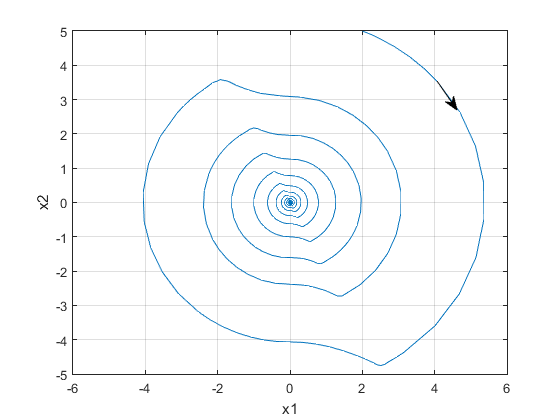
\includegraphics[width = 14 cm, height = 6 cm]{PlanoDeFaseQ4C05P1}
\caption{Mapa de Fase, x(0)=$[2~5]^T$, c=0.5}
\end{figure}
\begin{figure}
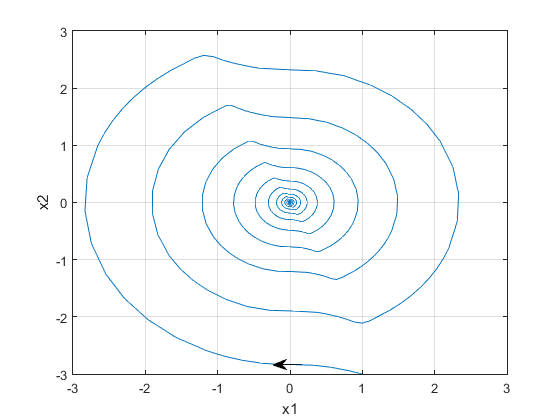
\includegraphics[width = 14 cm, height = 6 cm]{PlanoDeFaseQ4C05P2}
\caption{Mapa de Fase, x(0)=$[1~-3]^T$, c=0.5}
\end{figure}
\begin{figure}
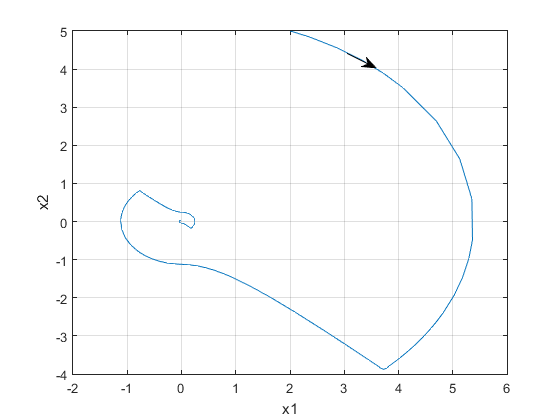
\includegraphics[width = 14 cm, height = 6 cm]{PlanoDeFaseQ4C10P1}
\caption{Mapa de Fase, x(0)=$[2~5]^T$, c=1}
\end{figure}
\begin{figure}
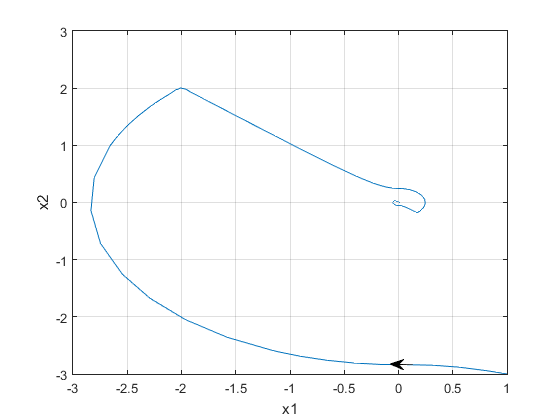
\includegraphics[width = 14 cm, height = 6 cm]{PlanoDeFaseQ4C10P2}
\caption{Mapa de Fase, x(0)=$[1~-3]^T$, c=1}
\end{figure}
\begin{figure}
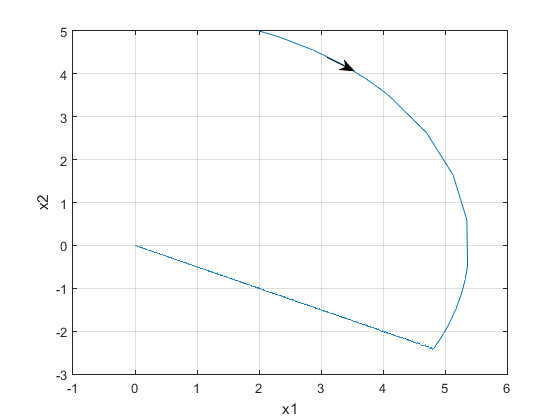
\includegraphics[width = 14 cm, height = 6 cm]{PlanoDeFaseQ4C20P1}
\caption{Mapa de Fase, x(0)=$[2~5]^T$, c=2}
\end{figure}
\begin{figure}
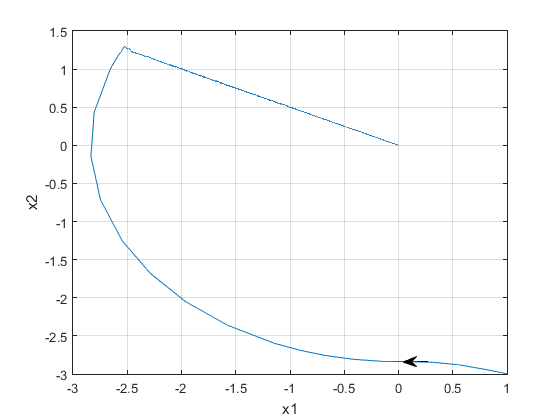
\includegraphics[width = 14 cm, height = 6 cm]{PlanoDeFaseQ4C20P2}
\caption{Mapa de Fase, x(0)=$[1~-3]^T$, c=2}
\end{figure}
\begin{figure}
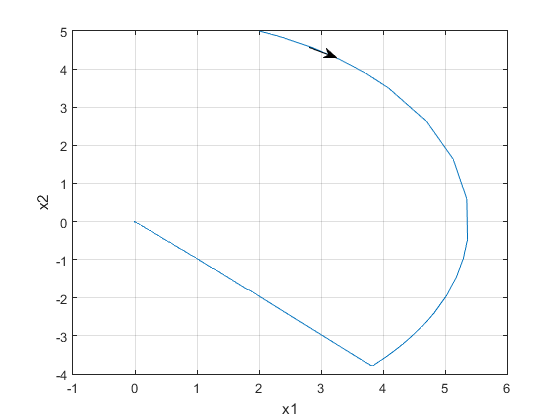
\includegraphics[width = 14 cm, height = 6 cm]{PlanoDeFaseQ4C103P1}
\caption{Mapa de Fase, x(0)=$[2~5]^T$, c=1.03}
\end{figure}
\begin{figure}
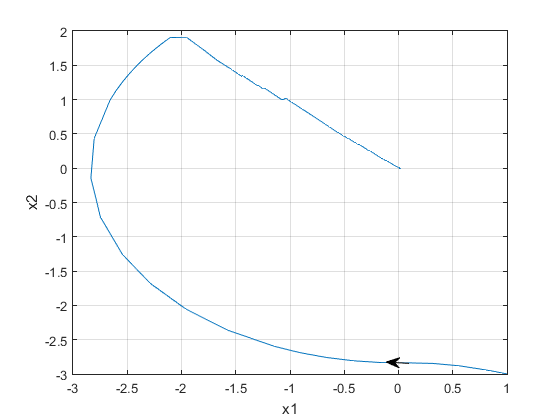
\includegraphics[width = 14 cm, height = 6 cm]{PlanoDeFaseQ4C108P2}
\caption{Mapa de Fase, x(0)=$[1~-3]^T$, c=1.08}
\end{figure}

\section{Questão 5}

a) Para o relé puro temos que $N(X) = \frac{4M}{\pi X}$. Para $G(jw)$ tal que $Im(G(jw))=0$ temos $G(jw)= \frac{K}{jw(1+jwT)(1+jwaT)}$, precisamos que $1-w^2aT^2=0$, que implica em $w=\frac{1}{\sqrt{a}T}$. Que leva a $x(t)=X\sin wt = \frac{4MKaT\sin(t/(\sqrt{a}T))}{\pi(1+a)}$. Como o cálculo feito foi literal e temos a garantia de que a>0, T>0 e K>0, sempre existirá ciclo limite.\\

b) Da letra a) temos $w=\frac{1}{\sqrt{a}T}$ e a amplitude $X=\frac{4MKaT}{\pi(1+a)}$.\\

c) Para $X<\frac{4MKaT}{\pi(1+a)}$ temos $G(jw)$ passando à esquerda do ponto -1/N(X) no eixo real, o que indica que a amplitude aumenta. Para $X>\frac{4MKaT}{\pi(1+a)}$ temos $G(jw)$ passando à direita do ponto -1/N(X) no eixo real, o que indica que a amplitude diminui. O ciclo limite é estável.\\

d)Alta frequência de oscilação e baixa amplitude.\\

e)Para K=M=T=1 e a=0.1 temos w=3.1623 para que $G(jw)$ intercepte o eixo real. Para que não haja ciclo limite, é necessário que a zona morta do relé invalide a equação $X=-GNX$, de forma que $-G(jw)N(X)\neq1$. O valor de $G(jw)$ que intercepta o eixo real é 0.1/1.1, caso a zona morta seja maior que este valor, não poderá haver ciclo limite.\\

f)Nas condições de e) basta calcular a atenuação para a segunda harmônica, caso o valor seja alto o suficiente a hipótese do filtro se mantém. Para w=6.3246 temos uma atenuação da ordem de $1/246 \approx 0.004$, a atenuação para a primeira harmônica é de aproximadamente 0.09, de forma que a primeira harmônica é atenuada aproximadamente 22 vezes menos que a segunda harmônica (~16dB). A hipótese do filtro se mantém.
\chapter{Lista de Exercício 3}
\section{Questão 1}
Questão 1) Para o sistema caracterizado por $\dot{x} = Ax$, temos que os autovalores da matriz $A$ são imaginários puros, $\pm jw$. Esta representação é equivalente a um oscilador linear sem amortecimento, tal que a solução $x(t)$ do sistema é uma senóide sem amortecimento. Pela definição de estabilidade colocada em sala, temos que o sistema é estável desde que a solução se mantenha numa vizinhança da origem sem se afastar, o que é o caso. 



\section{Questão 2}
Questão 2): Letra a) $V(x_1,x_2) = x_1^2 +x_1x_2+x_2^2+x_1x_2^3$ é indefinida, podendo ser colocada na forma $0.5(x_1 + x_2)^2 + 0.5x_1^2 + 0.5x_2^2 + x_1x_2^3$, tal que temos 3 termos com sinal definido positivo, mas existem condições em que o termo $x_1x_2^3$ domina os demais. Por exemplo $x_2=-1E10$ e $x_1=1$, cujo resultado é negativo\\

\noindent Letra b)$V(x_1,x_2) = x_1^2(1+x_2^2)$ é definida positiva. Não existem $x_1$ e $x_2$ que tornem V(x) negativa.\\ 

\noindent Letra c)$V(x_1,x_2) = x_1^2+x_2^4+x_2^3$ é indefinida, No intervalo entre -1 e 0 o termo indefinido $x_2^3$ domina o termo definido positivo $x_2^4$. De forma que existem combinações de $x_1$ qualquer e $x_2<0$ que tornam $V(x)<0$. Por exemplo $x_1 = 0$ e $x_2 = -0.1$.\\

\section{Questão 3}

Letra a) $\dot{x}_1 = 0$ implica em $x_1=0$ ou $x_1=2x_2$, $\dot{x}_2 = 0$ implica em $x_2=0$ ou $-2x_1+0.5-x_2=0$, para $x_1=0$ isto implica em $x_2=0.5$, para $x_1=2x_2$ isto implica em $x_2=0.1$ e $x_1=0.2$. Os pontos de equilíbrio do sistema são $[0~0]^T;[0~0.5]^T;[0.2~0.1]^T$.\\

Letra b) $\dot{x} = f(x)$, $\bar{x} = x - x^*$, $\dot{x}=f(\bar{x}+x^*)$. Para a origem não é preciso fazer translação. Para $[0.1~0.2]^T$ temos $\bar{x} = x - [0.1~0.2]^T$. $\dot{x}_1=f(\bar{x}_1+0.1,\bar{x}_2+0.2)$, $\dot{x}_2=f(\bar{x}_1+0.1,\bar{x}_2+0.2)$:
\begin{equation}
\dot{x}_1=-(\bar{x}_1+0.2)^2 + 2(\bar{x}_1+0.2)(\bar{x}_2+0.1) 
\end{equation}
\begin{equation}
\dot{x}_2=-2(\bar{x}_1+0.2)(\bar{x}_2+0.1) + 0.5(\bar{x}_2+0.1)-(\bar{x}_2+0.1)^2 
\end{equation} 

\noindent Da mesma forma, para $[0~0.5]^T$ temos:

\begin{equation}
\dot{x}_1=-(\bar{x}_1)^2 + 2(\bar{x}_1)(\bar{x}_2+0.5)
\end{equation}
\begin{equation}
\dot{x}_2=-2(\bar{x}_1)(\bar{x}_2+0.5) + 0.5(\bar{x}_2+0.5)-(\bar{x}_2+0.5)^2 
\end{equation} 

Letra c) Linearizando em torno dos respectivos pontos de equilíbrio temos para $[0~0]^T$:

\begin{equation}
\dot{x}_{1L}=0
\end{equation}
\begin{equation}
\dot{x}_{2L}=0.5x_2
\end{equation}

\noindent Para $[0.2~0.1]^T$:

\begin{equation}
\dot{x}_{1L}=-0.2\bar{x}_1 + 0.2\bar{x}_2
\end{equation}
\begin{equation}
\dot{x}_{2L}=-0.2\bar{x}_1 + 0.1\bar{x}_2
\end{equation}

\noindent Para $[0~0.5]^T$:

\begin{equation}
\dot{x}_{1L}=\bar{x}_1
\end{equation}
\begin{equation}
\dot{x}_{2L}=-\bar{x}_1 - 1.5\bar{x}_2
\end{equation}

Tal que, para $[0~0]^T$ somos levados à:

\begin{equation}
\begin{bmatrix}
0 & 0\\
0 & p_{22}
\end{bmatrix}
=
-Q
\end{equation}
\\

Que não tem solução e portanto concluímos que o ponto de equilíbrio é instável.\\

Para $[0~0.5]^T$ somos levados à:

\begin{equation}
\begin{bmatrix}
2 & -2 & 0\\
0 & -0.5 & -1\\
0 & 0 & -1.5
\end{bmatrix}
\begin{bmatrix}
p_{11}\\
p_{12}\\
p_{22}
\end{bmatrix}
=
\begin{bmatrix}
-q_{11}\\
-q_{12}\\
-q_{22}
\end{bmatrix}
\end{equation}

Cuja solução analítica é:

\begin{equation}
\begin{array}{l}
p_{11} = 2q_{12} - 2q_{22}/1.5 - q_{11}/2\\
p_{12} = 2q_{12} - 2q_{22}/1.5\\
p_{22} = q_{22}/1.5
\end{array}
\end{equation}

Sujeito a $P>0$ e $Q>0$, que nos leva à inequação ($\det Q>0$):

\begin{equation}
q_{11}q_{22}>q_{12}^2 
\end{equation}
Que resulta em:

\begin{equation}
0>(q_{22} - 0.375q_{11}/2)^2 + 2.25q_{11}^2/4 - 0.375^2q_{11}^2/4
\end{equation}

Cuja forma quadrática implica claramente numa contradição (os termos com sinal definido positivo claramente não podem ser negativos), e portanto o ponto de equilíbrio é instável, pois não é possível cumprir todas as condições.\\

Para $[0.2~0.1]^T$, somos levados à:

\begin{equation}
\begin{bmatrix}
-0.2p_{11} - 0.2p_{12} & 0.2p_{11}-0.1p_{12}-0.2p_{22}\\
0.2p_{11}-0.1p_{12}-0.2p_{22}& 0.2p_{12} + 0.1p_{22}
\end{bmatrix}
=
\begin{bmatrix}
-q_{11} & -q_{12}\\
-q_{12} & -q_{22}
\end{bmatrix}
\end{equation}

Que leva a:

\begin{equation}
\begin{bmatrix}
-0.4 & -0.4 & 0\\
0.2  & -0.1 & -0.2\\
0    & 0.4 &  0.2
\end{bmatrix}
\begin{bmatrix}
p_{11}\\
p_{12}\\
p_{22}
\end{bmatrix}
=
\begin{bmatrix}
-q_{11}\\
-q_{12}\\
-q_{22}
\end{bmatrix}
\end{equation}

Cuja solução analítica é:

\begin{equation}
\begin{array}{l}
p_{11}=7.5q_{11} + 10q_{12} + 10q_{22}\\
p_{12}=-5q_{11} - 10q_{12} - 10q_{22}\\
p_{22}= 10q_{11} +20q_{12} + 15q_{22}
\end{array}
\end{equation}

Escolhemos $q_{11} = 1$, $q_{22} = 1$, $q_{12} = -1$, tal que $P>0$, $Q>0$ e $\dot{V}(x) = -(x_1 - x_2)^2 <0$. O ponto de equilíbrio é estável.\\

Letra d) Apenas o ponto de equilíbrio estável possui domínio de estabilidade assintótica. A partir de nossa escolha para $V(x)$, chegamos a $\dot{V}(x) = -(x_1 - x_2)^2<0$ que implica que o domínio de estabilidade assintótico é todo o $\mathcal{R}^2$ para o ponto de equilíbrio $[0.2~0.1]^T$. No entanto, o sistema possui dois pontos de equilíbrio instáveis, de forma que nada se pode afirmar sobre o comportamento do sistema numa vizinhança destes pontos.\\

\section{Questão 4}

a) A condição dada equivale à seguinte escolha:

\[
-Q = \begin{bmatrix}
-2 & 0\\
0  & -2
\end{bmatrix}
\]

Tal que usando a equação de Lyapunov, para $k=1$, chegamos a:
\begin{equation}
\begin{bmatrix}
-1 & 1 & 0\\
-3 &-3 & 1\\
0  &-6 &-4
\end{bmatrix}
\begin{bmatrix}
p_{11}\\
p_{12}\\
p_{22}
\end{bmatrix}
=
\begin{bmatrix}
-1\\
 0\\
-2
\end{bmatrix}
\end{equation}

Como a matriz associada aos coeficientes de $P$ na equação tem posto cheio, chegamos a uma única solução, tal que:

\[
P = \begin{bmatrix}
2/3 & -1/3\\
-1/3 & 1
\end{bmatrix}
\]

Que leva à função $\dot{V}(x) = -2x_1^2 -2x_2^2<0$ e portanto o sistema é globalmente assintoticamente estável para $k=1$.\\

b) Partindo da matriz $P$ obtida na questão anterior, obtemos $\dot{V}(x) = x^T Q' x$:

\[
Q' = \begin{bmatrix}
-2k & 4k/3 - 4/3\\
4k/3 - 4/3 & 1
\end{bmatrix}
\]

E para que esta matriz tenha os autovalores no semiplano esquerdo são necessárias as seguintes condições:
\begin{equation}
k>0
\end{equation}
\begin{equation}
2k - (4k/3 - 4/3)^2 > 0
\end{equation}

E a segunda equação leva ao seguinte intervalo:

\begin{equation}
0.3619<k<2.7631
\end{equation}

Onde temos garantia de que o sistema é assintoticamente estável.

c) Para o sistema em questão os autovalores da matriz $A$ são: 

\begin{equation}
\lambda_{1,2} = \frac{-2 - k \pm \sqrt{k^2 - 16k +4}}{2}
\end{equation}

E basta que $-2 -k<0$ e que $|-2-k|>|\sqrt{k^2 - 16k +4}|$, que leva a:

\begin{equation}
k>0
\end{equation}

Que é necessário e suficiente. Podemos ver aqui a dificuldade em tratar com a teoria de estabilidade de Lyapunov comparada com o ferramental disponível para sistemas lineares, pois a escolha das funções de energia afeta diretamente a habilidade do analista de extrair resultados úteis enquanto que no caso dos sistemas lineares, possuímos uma maneira metódica e garantida de análise. Sabemos por exemplo que, dada a garantia em relação a $k$ o sistema acima é, além de assintoticamente, globalmente exponencialmente estável.  

\section{Questão 5}

Letra a) dado:\\

\begin{equation}
\dot{x} -0,5(x-2)x = 0
\end{equation}

\noindent Os pontos de equilíbrio são x=0 e x=2. x=0 é estável e atrativo na sua vizinhança e x=2 é instável:\\

\begin{equation}
V(x) = x^2
\end{equation}

\begin{equation}
\dot{V}(x) = 2x\dot{x} = x^2(x-2)
\end{equation}

\noindent $\dot{V}(x)$ é menor que 0 em torno de x=0. Enquanto que no segundo caso:\\

\begin{equation}
\dot{x} = 0.5(\bar{x}+2)\bar{x}
\end{equation}\

\begin{equation}
\dot{V}(\bar{x}) = 2\bar{x}\dot{\bar{x}} = \bar{x}^2(\bar{x}+2)
\end{equation}

\noindent $\dot{V}(x)$ é maior que 0 em torno de $x=2$.\\


Letra b), dado:\\

\begin{equation}
\ddot{x} + x^2 = 1(t)
\end{equation}

Em variáveis de estado:\\

\begin{equation}
x_1 = x
\end{equation}
\begin{equation}
x_2  = \dot{x}
\end{equation}
\begin{equation}
\dot{x_1} = x_2
\end{equation}
\begin{equation}
\dot{x_2} = -x_1^2+1(t)
\end{equation}

\noindent Cujos pontos de equilíbrio para t>0 são $[1~0]^T$ e $[-1~0]^T$, cujas equações ajustadas são, para $[1~0]^T$:\\

\begin{equation}
\dot{x_1} = \bar{x_2}
\end{equation}
\begin{equation}
\dot{x_2} = -(\bar{x_1}+1)^2+1(t) = -\bar{x_1}^2 - 2\bar{x_1}
\end{equation}

\noindent E para $[-1~0]^T$:\\

\begin{equation}
\dot{x_1} = \bar{x_2}
\end{equation}
\begin{equation}
\dot{x_2} = -(\bar{x_1}-1)^2+1(t) = -\bar{x_1}^2 + 2\bar{x_1}
\end{equation}

Linearizando cada par de equações encontramos os seguintes sistemas:

\[
\dot{x} = \begin{bmatrix}
0 & 1\\
-2 & 0
\end{bmatrix} x
\]

Que é estável apenas no sentido de saída limitada.

\[
\dot{x} = \begin{bmatrix}
0 & 1\\
2 & 0
\end{bmatrix}x
\]

Que é instável.

\section{Questão 6}

a) Seja o sistema linearizado em torno da origem, como $h_1(0) = h_2(0) = 0$, temos:

\begin{equation}
\dot{x}_{1L} = -\frac{\partial h1(x_1)}{\partial x_1} \bigg |_{x_1 = 0} x_1+\frac{\partial h2(x_2)}{\partial x_2} \bigg |_{x_2 = 0} x_2
\end{equation}

\begin{equation}
\dot{x}_{2L} = x_1 - ax_2
\end{equation}

Tal que a matriz $A$ do sistema linearizado $\dot{x}_L = Ax_L$ é:

\[
A = \begin{bmatrix}
 -\frac{\partial h1(x_1)}{\partial x_1} \bigg |_{x_1 = 0} & \frac{\partial h2(x_2)}{\partial x_2} \bigg |_{x_2 = 0}\\
 1 & -a
\end{bmatrix}
\]

E basta que seus autovalores pertençam ao semiplano esquerdo. Fazemos a notação:
\[
 \frac{\partial h1(x_1)}{\partial x_1} \bigg |_{x_1 = 0} \equiv h_1^{'}(0)
 \] \\ 
 \[\frac{\partial h2(x_2)}{\partial x_2} \bigg |_{x_2 = 0} \equiv h_2^{'}(0)
\]


Que leva às seguintes condições:
\begin{equation}
h_1^{'}(0)a - h_2^{'}(0) >0
\end{equation}
\begin{equation}
a>0
\end{equation}
\begin{equation}
h_1^{'}(0)>0
\end{equation}

b)Utilizando o teorema de Krasovskii, calculamos a matriz:

\[
M = \begin{bmatrix}
 2(-h_1(x1) + h_2(x2))\frac{\partial h1(x_1)}{\partial x_1} & -1 -(x_1-ax_2)\frac{\partial h2(x_2)}{\partial x_2}\\
-1 -(x_1-ax_2)\frac{\partial h2(x_2)}{\partial x_2} & 2a
\end{bmatrix}
\]

E usando a mesma notação da letra a) e omitindo o argumento de $h_1(x1)$ e $h_2(x2)$, temos:

\[
M = \begin{bmatrix}
 2(-h_1 + h_2)h_1^{'} & -1 -(x_1-ax_2)h_2^{'}\\
-1 -(x_1-ax_2)h_2^{'} & 2a
\end{bmatrix}
\]

É necessário que os autovalores da matriz pertençam sempre ao semiplano esquerdo, tal que:

\begin{equation}
(-h_1 + h_2)h_1^{'}>0,~~\forall x_1,x_2
\end{equation}
\begin{equation}
a>0
\end{equation}
\begin{equation}
4a(-h_1 + h_2)h_1^{'} - (-1 -(x_1-ax_2)h_2^{'})^2 >0~~\forall x_1,x_2
\end{equation}

São as condições necessárias e suficientes para estabilidade assintótica global. 

\section{Questão 7}
Dado:

\begin{equation}
\dot{x} = -\sin x
\end{equation}

a) Temos que os pontos de equilíbrio são da forma $x=n\pi$, $n\in \mathcal{Z}$. A linearização para estes pontos produz a seguinte equação:

\begin{equation}
\dot{\bar{x}} = \cos (n\pi)*(\bar{x})
\end{equation}

Com $\bar{x} = x-n\pi$\\

De forma que:

\begin{equation}
V(\bar{x}) = \bar{x}^2/2
\end{equation}

E:

\begin{equation}
\dot{V}(\bar{x}) = \bar{x}^2*\cos(n\pi)
\end{equation}

Os pontos com n ímpar são atrativos e os pontos com n par são instáveis, pois $\cos(n\pi)$ determina o sinal de $\dot{V}$.\\

Letra b) O limite de senx/x quando x tende a 0 é 1. x=0 é instável.\\

Letra c) Seja $V(x) = \int_{0}^{x} f(\tau) d\tau = -(\cos x-\cos 0) = 1 - \cos x$, que é apenas semi definida positiva dentro do intervalo, sua derivada resulta em:\\

\begin{equation}
\dot{V}(x) = - \sin^2 x < 0
\end{equation}

Porém, como o sistema possui múltiplos pontos de equilíbrio, o comportamento assintótico em relação à origem não fica muito bem especificado, sabemos que numa vizinhança da origem existe estabilidade assintótica, mas não sabemos qual é esta vizinhança, já que os teoremas estudados requerem $V(x)$ definida positiva na maioria dos casos.\\ 

Letra d) $-\pi<x<\pi$, (enquanto $\pi>x>0$ temos $f(x)<0$ e x retorna à origem, enquanto $0>x>-\pi$ temos $f(x)>0$ e x também retorna à origem, ambos sem chance de serem atraídos por pontos de equilíbrio vizinhos, já que estes são instáveis)\\

\section{Questão 8}

Seja $\dot{x} = Ax$, com:

\[A = 
\begin{bmatrix}
   0 & 1 \\
  -1 & -2
\end{bmatrix}
\]

Escolhemos:

\[Q = \begin{bmatrix}
    -1 & -1\\
    -1 & -1
\end{bmatrix}
\]

Tal que, resolvendo para P, obtemos:

\[\begin{bmatrix}
    -1 & -1\\
    -1 & -1
\end{bmatrix}
=
\begin{bmatrix}
-2p_{12} & -p_{22} + p_{11} - 2p_{12}\\
-p_{22} + p_{11} - 2p_{12} & 2p_{12} - 4p_{22}
\end{bmatrix}
\]

tal que:

\[
P = \begin{bmatrix}
 1/2 & 1/2 \\
 1/2 & 1/2
\end{bmatrix}
\]

seja a candidata $V(x) = x^T P x$ que leva a $\dot{V}(x) = -x^TQx$, temos que:

\begin{equation}
\dot{V}(x) = -2V(x)
\end{equation}

E portanto a energia do sistema decai com uma constante de tempo igual a 2. Poderíamos estimar o transitório usando a inequação $||x||^2 \lambda_{max,P}\geq x^TPx\leq ||x||^2 \lambda_{min,P}$, de forma que teriamos uma inequação envolvendo $\dot{V}(x)/V(x) \leq \lambda_{min,q}/\lambda_{max,p}$, porém, como nossa escolha de $Q$ resultou, fortuitamente, em $P$ linearmente dependente de $Q$, chegamos a um resultado exato e o uso da inequação não foi necessário.

\end{document}         